\newpage
\subsection{Introduction to the Optimal Control Problem}
\noindent To optimize the ollie and the geometry of the skateboard, the observations from the previous section should be modeled numerically with physics and mathematics. Before the physical ollie phenomena are discussed, the chosen optimization scheme is introduced. 

\subsubsection{Optimal Control}\label{s_optimalcontrol}
\noindent There are three types of optimizations to solve an optimal control problem (OCP) \cite{kelly_transcription_2017}:
\begin{itemize}
    \item \textbf{Dynamic programming} - This type of optimization discretizes the whole solution space and finds the global optimum. A perfect method for a low dimensional system. But when scaling to a high dimensional system the computation time will increase exponentially. 
    \item \textbf{Indirect methods} - Transcribe the problem and find where the slope of the objective is zero. Often numerically unstable and difficult to implement and initialize.
    \item \textbf{Direct methods} - Transcribe the problem then find the minimum of the objective function. Can transcribe well to high dimensional systems, but is prone to finding a local optima because it searches a single trajectory through state and control space rather than a global method like dynamic programming.
\end{itemize}
I chose the direct method, because direct methods are generally best for problems where dynamics and control must be computed to a similar accuracy, and the structure of the control trajectory is not known a priori \cite{kelly_introduction_2017}. Also, the ollie is highly non-linear and complex movement with high dimensionality . With this method it is possible to increase the dimensionality without increasing the difficulty to solve the optimization. 

\subsubsection{Transcription and Mesh}
\noindent Transcription is converting a continuous problem into a non-linear programming problem (NLP). There are shooting methods and simultaneous methods. A shooting method uses a simulation to enforce the system dynamics, while the simultaneous method enforces the dynamics at given points along the trajectory. The chosen method is a simultaneous method called orthogonal collocation. The software that is used is called PyCollo, which is direct orthogonal collocation transcription tool for Python \cite{brockie_predictive_nodate}. The dynamics and constraints are enforced over a discretization. The discretization exists of $N$ collocation points. The collocation points are either mesh points or polynomial points, but all collocation points are enforced to the constraints and dynamics. After transcription the problem is passed to the solver IPOPT (Interior Point OPTimizer). When the found IPOPT solution does not meet the error-tolerance set in PyCollo, the discretization is refined and a new iteration is solved in IPOPT. Mesh points, polynomial points, mesh sections and mesh refinement are explained in figure \ref{f_phmesh}. The polynomials are of the Legendre-Gauss-Lobatto (LGL) nature. More information on the mesh can be found in appendix A. The integration scheme is an implicit Runge-Kutta Kth method \cite{brockie_predictive_nodate}. This high order method will have a high accuracy with the disadvantage that all states and constraints need to be differentiable.

\begin{figure}
    \centering
    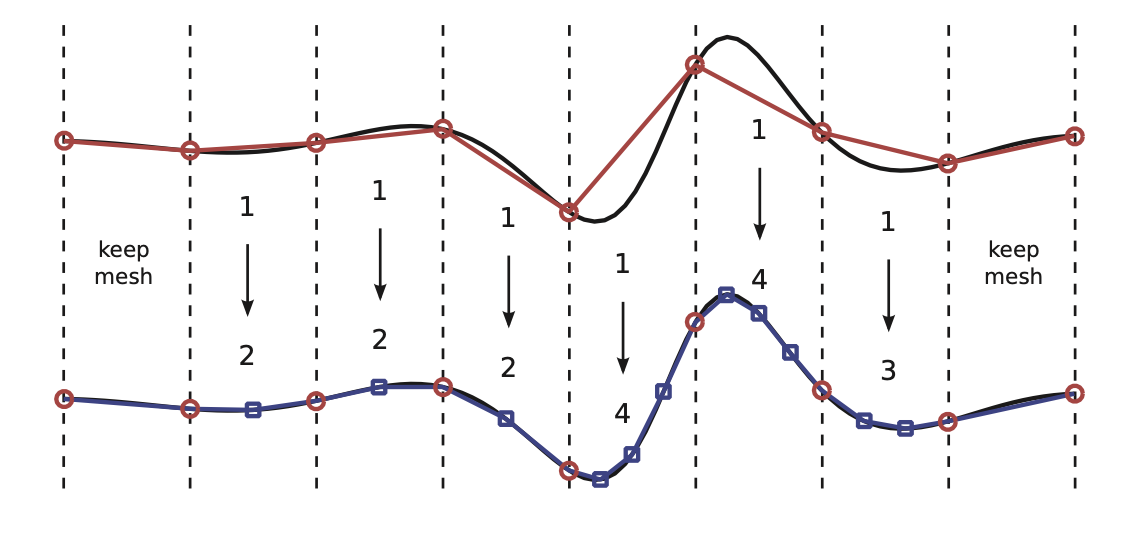
\includegraphics[width = 0.5\textwidth]{figure/phmesh.png}
    \caption[Mesh section and polynomials]{Mesh sections are indicated with the dotted vertical lines. The first line shows an optimization solution (red line) that has an error from the true solution (black line). With the increase of polynomial points the mesh is refined and the solution is better after a new iteration into IPOPT. If polynomial points exceed the limit of 10 points per mesh section, the mesh section will be made smaller. Highly nonlinear sections will refine more giving an efficient computation}
    \footnotesize Source: \cite{kelly_introduction_2017}
    \label{f_phmesh}
\end{figure}

\subsubsection{Hybrid problem}
\noindent The ollie problem is a hybrid problem, meaning that there will be discontinuities in the states. For example during impact the velocity states change sign instantly causing discontinuities. Discontinuities are per definition not differentiable, this means that in a higher order optimization the discontinuity need to be solved differently. The chosen method is to implement a multi-phase optimization. Multi-phase optimization concerns a sequence of continuous-state phases separated by discrete jumps in the states. Multi-phase optimization requires pre-modeled phases which leaves no opportunity for unsought solutions. Though, they are easier to compute and tend to be more accurate \cite{kelly_introduction_2017}. Since the impact is prescribed in the ollie, solving the impact velocities discretely will provide an accurate solution.

% The mechanics of the ollie show discontinuous behaviour, such as impact and friction. This usually leads to bad convergence for the solver. The solution is to change the system dynamics. For example, to discribe discontinous phenomena as continuous or split the problem up in several phases that are fully continuous or a combination of both. Impact can be solved with through-contact optimization. This is a continuous approximation of impact where contact mechanics are modeled with spring damper models.  The friction contact is not known in the ollie problem and can change throughout the whole movement. This is why a continuous approximation is chosen for the friction shown by equation \ref{e_friction}.